\clearpage
\VerdierPhysicalPageAnchor{0101}%
\begingroup
\small
\setlength{\abovedisplayskip}{3pt plus 2pt minus 2pt}%
\setlength{\belowdisplayskip}{3pt plus 2pt minus 2pt}%
\setlength{\jot}{2pt}%
\VerdierSemanticAnchor{ch1-3-3-6-two-arrow-object}
Soit maintenant
$i\xrightarrow{f}j\xrightarrow{g}k$ un objet de
$\mathcal{F}\ell_2(\mathcal{J})$. On peut lui faire correspondre le diagramme
suivant de $\operatorname{Tr}_1(C)$ :

\VerdierSemanticAnchor{ch1-3-3-6-2}
\begin{equation}
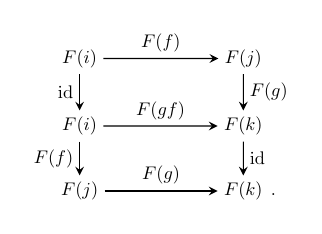
\begin{tikzpicture}[>=stealth,baseline=(current bounding box.center),scale=0.66,
  every node/.style={transform shape}]
  \node (Fi1) at (0,2.55) {$F(i)$};
  \node (Fj1) at (3.15,2.55) {$F(j)$};
  \node (Fi2) at (0,1.25) {$F(i)$};
  \node (Fk1) at (3.15,1.25) {$F(k)$};
  \node (Fj2) at (0,0) {$F(j)$};
  \node (Fk2) at (3.15,0) {$F(k)$};
  \draw[->] (Fi1) -- node[above] {$F(f)$} (Fj1);
  \draw[->] (Fi2) -- node[above] {$F(gf)$} (Fk1);
  \draw[->] (Fj2) -- node[above] {$F(g)$} (Fk2);
  \draw[->] (Fi1) -- node[left] {$\mathrm{id}$} (Fi2);
  \draw[->] (Fj1) -- node[right] {$F(g)$} (Fk1);
  \draw[->] (Fi2) -- node[left] {$F(f)$} (Fj2);
  \draw[->] (Fk1) -- node[right] {$\mathrm{id}$} (Fk2);
  \node[anchor=base west,inner sep=0pt,xshift=.08em] at (Fk2.base east) {$.$};
\end{tikzpicture}
\tag{3.3.6.2}
\end{equation}

\VerdierSemanticAnchor{ch1-3-3-6-delta}
Posons :
\begin{equation}
\begin{aligned}
  \delta(f,g)&\colon S(g)\longrightarrow S(f)[1],\\
  \delta(f,g)&=\dot p(F(f))[1]\dot q(F(g)).
\end{aligned}
\tag{3.3.6.3}
\end{equation}
En appliquant le foncteur cône au diagramme (3.3.6.2), on obtient un foncteur
de $\mathcal{F}\ell_2(\mathcal{J})$ dans la catégorie des triangles de
$K(C)$ :

\VerdierSemanticAnchor{ch1-3-3-6-4}
\begin{equation}
  \bigl(i\xrightarrow{f}j\xrightarrow{g}k\bigr)
  \longmapsto
  S(f)\longrightarrow S(gf)\longrightarrow S(g)
  \xrightarrow{\delta(f,g)}S(f)[1].
  \tag{3.3.6.4}
\end{equation}
\VerdierSemanticAnchor{ch1-3-3-6-distinguished-conclusion}
La fin de la démonstration de (3.3.5) montre que le triangle
\[
  S(f)\longrightarrow S(gf)\longrightarrow S(g)
  \xrightarrow{\delta(f,g)}S(f)[1]
\]
est un triangle distingué.

\VerdierSemanticAnchor{ch1-3-4}
\subsection{Propriétés fonctorielles des triangles distingués}

\VerdierSemanticAnchor{ch1-3-4-1}
\noindent\textbf{Proposition 3.4.1.}\quad
Soient
$\iota_1\colon K(C)^{\circ}\longrightarrow K(C^{\circ})$
l'isomorphisme canonique (2.5.13) et
\[
  X\xrightarrow{u}Y\xrightarrow{v}Z\xrightarrow{w}X[1]
\]
un triangle distingué de $K(C)$. Le triangle de $K(C^{\circ})$
\VerdierSemanticAnchor{ch1-3-4-1-opposite-triangle}
\[
  (\iota_1X)[-1]\xrightarrow{\iota_1w}\iota_1Z
  \xrightarrow{\iota_1v}\iota_1Y
  \xrightarrow{-\iota_1u}\iota_1X
\]
est distingué.
\endgroup

